\section{Kapitel 1}
\subsection{Unterkapitel 1.1}
\subsubsection{Unterunterkapitel 1.1.1}

%
\piccaption{Darstellung des Zahlenbereichs des Zweierkomplements mit acht Stellen\label{fig:tabelle_zweierkomplement}}
\parpic[r]{%
  \fbox{
    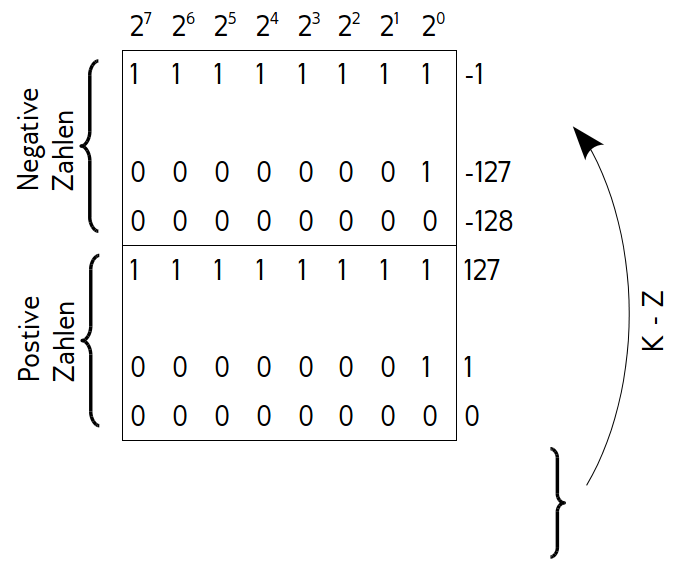
\includegraphics[width = 5.5cm, keepaspectratio]{images/tabelle_zweierkomplement.png}
  }
}
%
Die gängigste Form der Zahlensysteme sind Stellenwertsysteme. Eine Zahl $a$ wird in Form einer Reihe von Ziffern $z_i$ mit dazugehöriger Potenz der Basis $b^i$ dargestellt. Der Wert der Zahl ergibt sich dann als Summe der Werte aller Einzelstellen: $a = \sum\limits_{i}z_ib^i$.

\textbf{Umrechnung} in andere Zahlensysteme: Gegeben sei Zahl $Z$, umzuwandeln in System mit Basis $b$.
Eine angenehme Vorgehensweise gibt uns das \textbf{Horner Schema}\footnote{
Website mit Umrechnungen und Erklärungen: \url{http://www.arndt-bruenner.de/mathe/scripts/Zahlensysteme.htm}
}: Dividiere $Z$ durch $b$. Der Rest dieser Division ist die letzte Stelle der Zahl in der Basis $b$  (Einerstelle). Dividiere den Quotienten dieser Division wieder durch $b$. Der Rest dieser zweiten Division ergibt die zweite Stelle der Zahl in der neuen Basis. Wiederhole Divisionen, bis kein Rest mehr.